\documentclass{article}
\usepackage[utf8]{inputenc}
\usepackage[backend=biber]{biblatex}
\usepackage{amssymb}
\usepackage{amsmath}
\usepackage{dsfont}
\addbibresource{bib.bib}
\setlength{\parindent}{0em}
\bibliography{bib}
\setlength{\parskip}{6pt}
\usepackage[margin=1.0in]{geometry}
\usepackage{graphicx}
\usepackage{caption}
\usepackage{subcaption}
\usepackage{wrapfig}
\usepackage{url}

\title{Intro to deep learning with PyTorch}
\author{Miguel A. Saavedra-Ruiz}
\date{May 2020}
\linespread{1.0}

\nocite{*}


\begin{document}

\maketitle

\section*{Convolutional Neural Networks}

Convolutional Neural Networks (CNNs) are a variation of neural networks with the ability to efficiently operate over images. CNNs can look at images as a whole and learn to identify spatial patterns such as prominent colors and shapes, or whether a texture is fuzzy or smooth and so on. The shapes and colors that define any image and any object in an image are often called \textbf{features} Fig. \ref{fig:f1}.

An example of a feature would be what do we look at to distinguish a cat and a dog. These characteristics might be the shape of the eyes, the size, and how they move are just a couple of examples of visual features. 

\begin{figure}[ht]
    \centering
    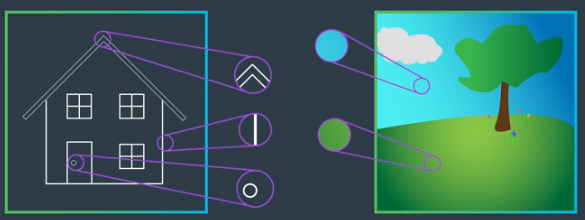
\includegraphics[width=0.45\textwidth,height=0.45\textheight,keepaspectratio]{images/features.png}
    \captionsetup{justification=centering}
    \caption{Features in an image}
    \label{fig:f1}
\end{figure}

To understand neural networks, it is important to also understand how an image is represented in a computer. In the case of gray scale images, these are interpreted by a computer as an array. A grid of values for each grid cell is called a pixel, and each pixel has a numerical value. In the MNIST database, each image is 28 pixels height and wide. Therefore, these images are understood by a computer as a 28 by 28 array. In a typical gray scale image, white pixels are encoded as the value 255, and black pixels are encoded as zero. Gray pixels fall somewhere in between, with light-gray being closer to 255. This description can be easily undertood with Fig. \ref{fig:f2}

\begin{figure}[ht]
    \centering
    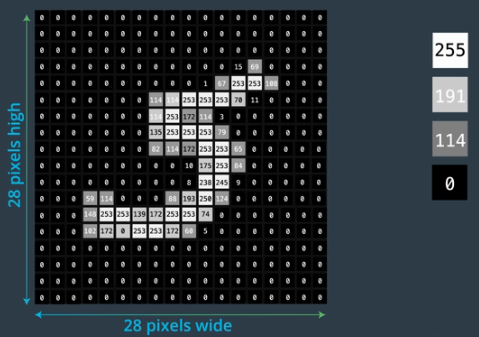
\includegraphics[width=0.4\textwidth,height=0.4\textheight,keepaspectratio]{images/image_representation.png}
    \captionsetup{justification=centering}
    \caption{Image representation as a matrix}
    \label{fig:f2}
\end{figure}

Nevertheless, the images in the MNIST dataset have actually gone through a quick pre-processing step. They've been re-scaled so that each image has pixel values in a range from zero to one Fig. \ref{fig:f3}. To go from a range of 0-255 to zero and one, it is necessary to divide every pixel value by 25 Eq. \eqref{eq:1}5. This step is called \textbf{normalization}.

\begin{figure}[ht]
    \centering
    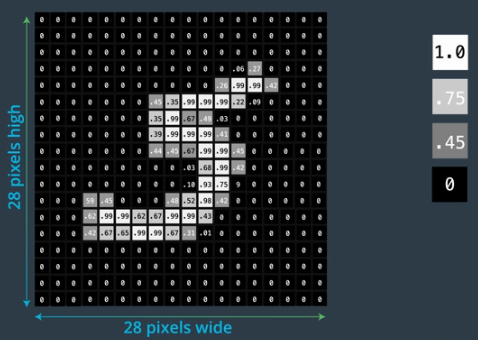
\includegraphics[width=0.4\textwidth,height=0.4\textheight,keepaspectratio]{images/image_norm.png}
    \captionsetup{justification=centering}
    \caption{Image representation as a normalized matrix}
    \label{fig:f3}
\end{figure}

\begin{equation}
NormX_{ij} = \frac{X_{ij}}{max(X)} \label{eq:1}
\end{equation}

Normalization is a useful tool to help the algorithm to train better. Thiss tep is quite useful due to neural networks rely on gradient calculations. These networks are trying to learn how important or how weighty a certain pixel should be in determining the class of an image. Normalizing the pixel values helps these gradient calculations stay consistent, and not get so large that they slow down or prevent a network from training.

Recall that to classify objects, the most common technique used for this was to use a MLP or fully connected neural network. However, these networks require 1-dimensional data. Hence, it is necessary to convert any array image into a vector. This process is called \textbf{flattening} and can be seen in Fig. \ref{fig:f4}. In this example, a four-by-four image which is a matrix with 16 pixel values. Instead of representing this as a four-by-four matrix, it is possible to construct a vector with 16 entries, where the first first entries of the vector correspond to the first row of the old array. The second four entries correspond to the second row and so on.

\begin{figure}[ht]
    \centering
    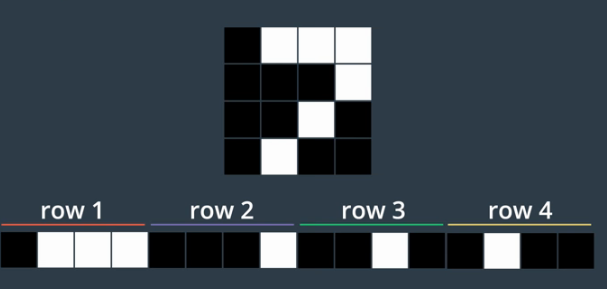
\includegraphics[width=0.4\textwidth,height=0.4\textheight,keepaspectratio]{images/flattening.png}
    \captionsetup{justification=centering}
    \caption{Flattening a simple matrix into a vector}
    \label{fig:f4}
\end{figure}

Once an image has been flattened, it is easy to pass the data to a MLP and obtain the classification result of the image.

It is important to note that Pytorch does Data normalization by subtracting the mean (the average of all pixel values) from each pixel, and then dividing the result by the standard deviation of all the pixel values.

\[\frac{P_{ij} - \mu}{\sigma}\]

Where for \(\mu = 0.5\) and \(\sigma=0.5\) the minimum (pixel coordinate equals 0) and maximum (pixel coordinate equals 1) values of the normalization are.

\[\frac{1 - 0.5}{0.5} = 1\]
\[\frac{0 - 0.5}{0.5} = -1\]

Resulting in a normalization of \([-1,1]\) for all the pixel values in the image.

A feasible network architecture to train the neural network is the one presented in Fig. \ref{fig:f50}. A MLP with 784 input units (number of inputs after flattening a MNIST image), two hidden layers with 512 nodes each and 10 output layers with a softmax activation function (one output per character) to produce a probability distribution in the final layer of the network.

\begin{figure}[ht]
    \centering
    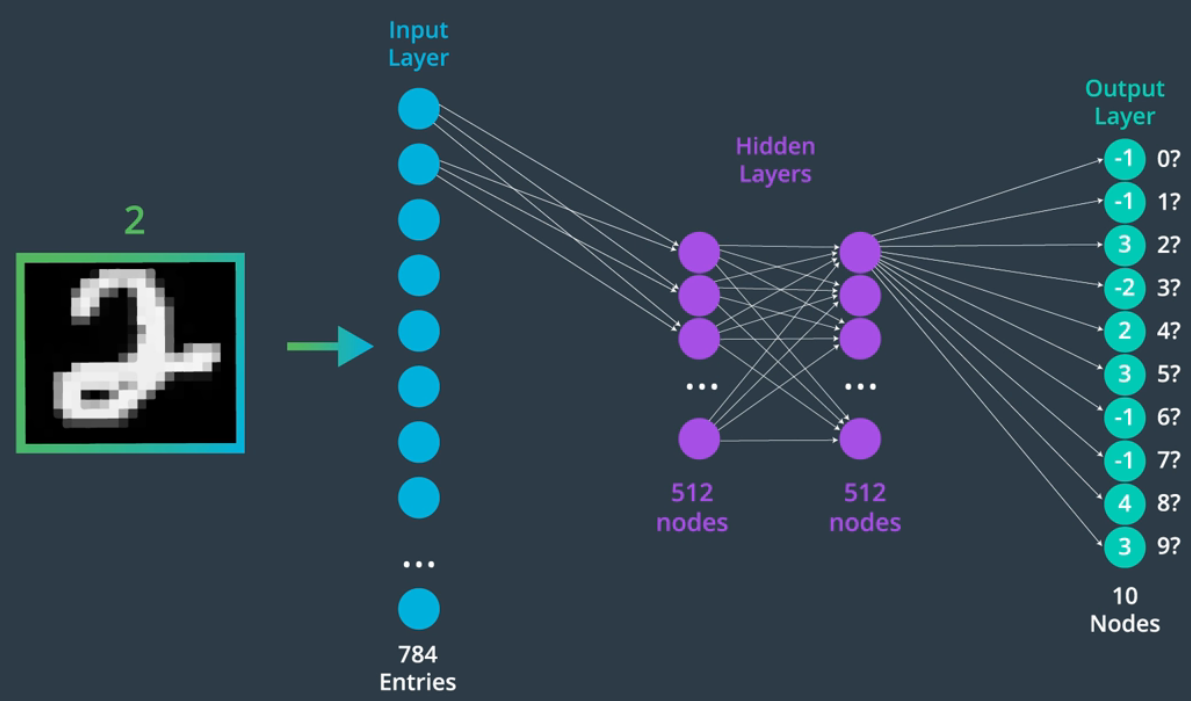
\includegraphics[width=0.55\textwidth,height=0.55\textheight,keepaspectratio]{images/mlp.png}
    \captionsetup{justification=centering}
    \caption{MLP to train a MNIST image}
    \label{fig:f5}
\end{figure}

Recall that neural networks learn from mistakes, hence, the next list of stems gives a gives of how to optimize the weights of a neural network.

\begin{enumerate}
  \item Loss: Measure any mistake between a predicted and true class
  \item Backpropagation: Quantify how bad a particular weight is in making a mistake
  \item Optimization: Gives a way to calculate a better weight value
\end{enumerate}

As this problem is categorized as a multi-classes problem, the \textbf{loss function} needed is called \textbf{categorical cross-entropy loss}. This loss function is defined as the negative log of the output layer (with softmax activation function).

Therefore, if the probability of a node is \(p(x_i) = 0.162\) the negative log is given in Eq. \eqref{eq:2}.

\begin{equation}
loss = -\log(0.162) = 1.82 \label{eq:2}
\end{equation}

If the probability is something like \(p(x_i) = 0.441\), then the loss would be \(loss = 0.819\)

It is possible to conclude that the categorical cross-entropy loss is \textbf{lower} when the prediction and label agree and \textbf{higher} when the prediction and label disagree (a probability close to one yields to a low loss value).

The optimizer is used to minimize the error of the loss function and change the weights towards the minimum error expression. In the Fig. \ref{fig:f6}, in the top right box it is possible to see a list of different optimizer and their performance minimizing the error. Each optimizer has its own benefits and the selection of one or other depends on the problem.

\begin{figure}[ht]
    \centering
    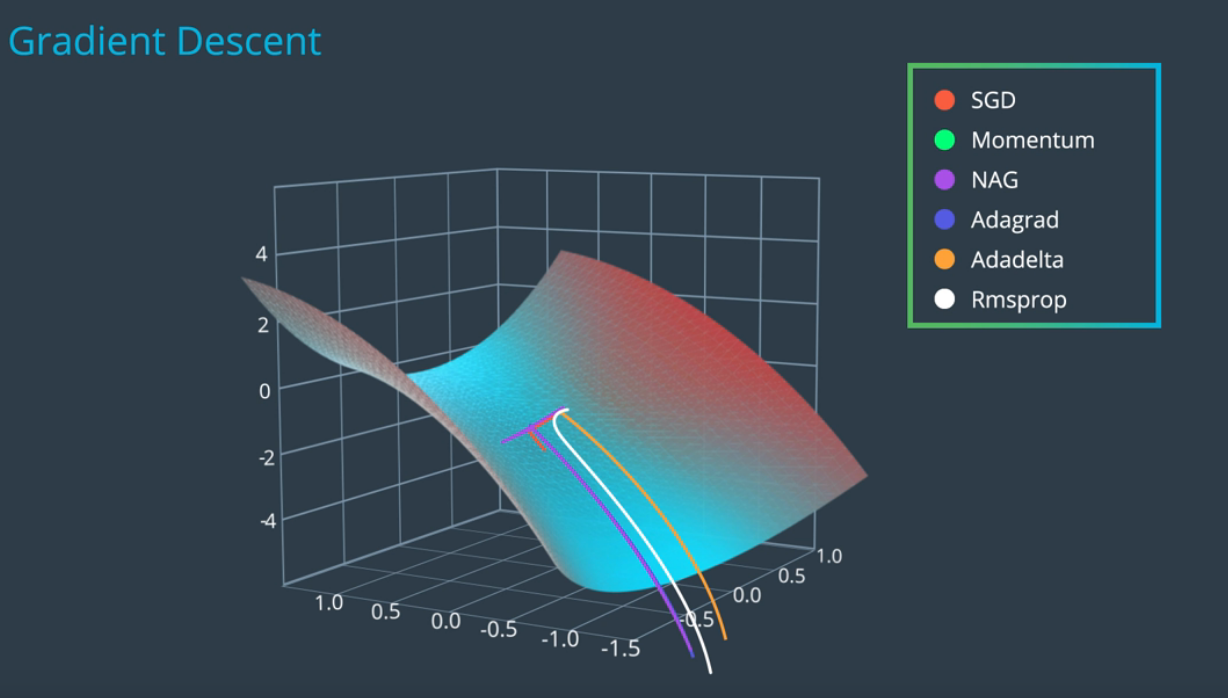
\includegraphics[width=0.4\textwidth,height=0.4\textheight,keepaspectratio]{images/optimizer.png}
    \captionsetup{justification=centering}
    \caption{Optimizer used to train a neural network}
    \label{fig:f6}
\end{figure}

A complete solution to the problem described before can be seen in \textit{mnist\_mlp\_exercise.ipynb}.

To decide whether the model is doing well or bad during training, a new set needs to be introduced. \textbf{The validation set} is defined as a sub-sample of the training set, usually the 20\% of the training set. During training, the training set is used to change the weights and the validation set checks the performance of the model to avoid over-fitting. Finally, once a model has been chosen, a test set is used (this set has never been seen by the network before) to check the accuracy of the trained model. The pipeline described before can be seen in Fig. \ref{fig:f7}.

\begin{figure}[ht]
    \centering
    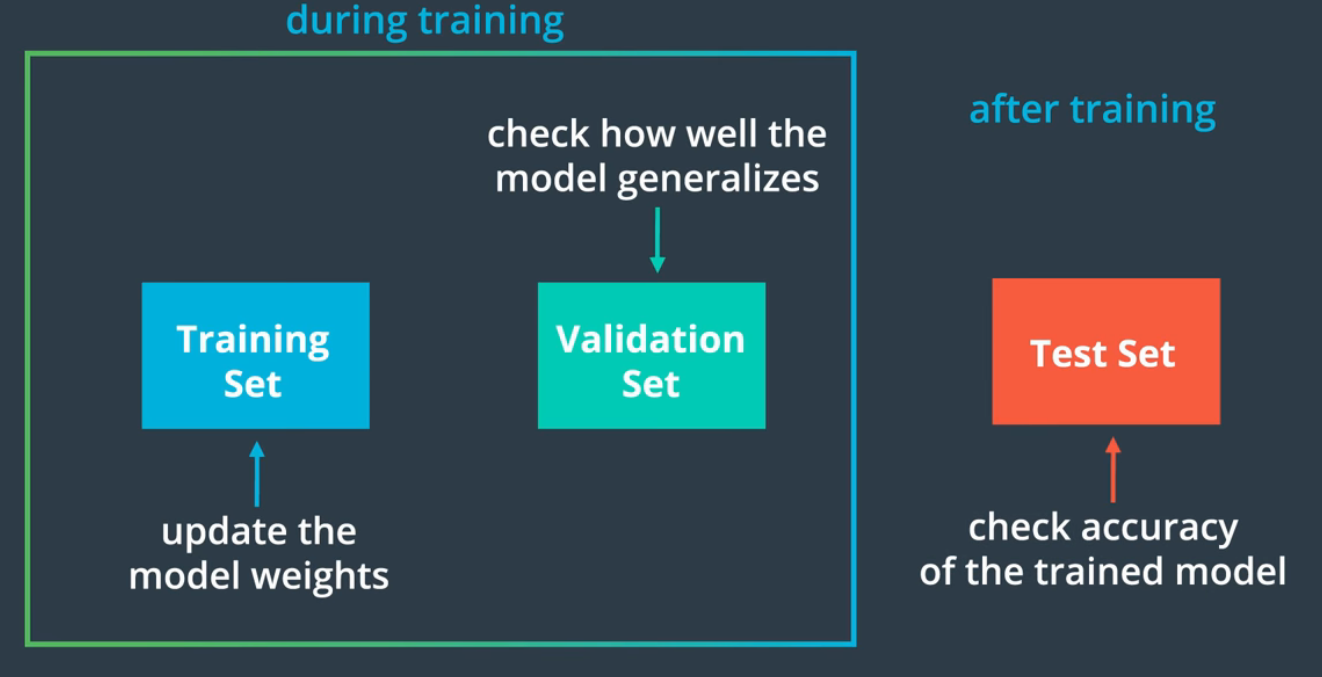
\includegraphics[width=0.55\textwidth,height=0.55\textheight,keepaspectratio]{images/sets.png}
    \captionsetup{justification=centering}
    \caption{Sets the evaluate and train a model}
    \label{fig:f7}
\end{figure}


\printbibliography

\end{document}

